\documentclass[]{final_report}
\usepackage{graphicx}
\usepackage{hyperref}
\usepackage{listings}
\usepackage{svg}
\usepackage{afterpage}
\usepackage{pdflscape}
\usepackage{amsmath}
\usepackage{algpseudocode}

\usepackage{color}
\definecolor{lightgray}{rgb}{.9,.9,.9}
\definecolor{darkgray}{rgb}{.4,.4,.4}
\definecolor{purple}{rgb}{0.65, 0.12, 0.82}
\lstdefinelanguage{JavaScript}{
  keywords={break, case, catch, continue, debugger, default, delete, do, else, false, finally, for, function, if, in, instanceof, new, null, return, switch, this, throw, true, try, typeof, var, void, while, with},
  morecomment=[l]{//},
  morecomment=[s]{/*}{*/},
  morestring=[b]',
  morestring=[b]",
  ndkeywords={class, export, boolean, throw, implements, import, this},
  keywordstyle=\color{blue}\bfseries,
  ndkeywordstyle=\color{darkgray}\bfseries,
  identifierstyle=\color{black},
  commentstyle=\color{purple}\ttfamily,
  stringstyle=\color{red}\ttfamily,
  sensitive=true
}

\lstset{
   language=JavaScript,
   backgroundcolor=\color{lightgray},
   extendedchars=true,
   basicstyle=\footnotesize\ttfamily,
   showstringspaces=false,
   showspaces=false,
   numbers=left,
   numberstyle=\footnotesize,
   numbersep=9pt,
   tabsize=2,
   breaklines=true,
   showtabs=false,
   captionpos=b
}

%%%%%%%%%%%%%%%%%%%%%%
%%% Input project details
\def\studentname{Arran France}
\def\reportyear{2018}
\def\projecttitle{Array Support for Dynamic Symbolic Execution of JavaScript}
\def\supervisorname{Dr Johannes Kinder}
\def\degree{BSc (Hons) in Software Engineering}
\def\fullOrHalfUnit{Full Unit} % indicate if you are doing the project as a Full Unit or Half Unit
\def\finalOrInterim{Final Report} % indicate if this document is your Final Report or Interim Report

\begin{document}

\maketitle

%%%%%%%%%%%%%%%%%%%%%%
%%% Declaration

\chapter*{Declaration}

This report has been prepared on the basis of my own work. Where other published and unpublished source materials have been used, these have been acknowledged.

\vskip3em

Word Count: 18,038

\vskip3em

Student Name: \studentname

\vskip3em

Date of Submission: 2018-03-28

\vskip3em

Signature: Arran France

\newpage

%%%%%%%%%%%%%%%%%%%%%%
%%% Table of Contents
\tableofcontents\pdfbookmark[0]{Table of Contents}{toc}\newpage

%%%%%%%%%%%%%%%%%%%%%%
%%% Your Abstract here

\begin{abstract}

%TODO Write abstract

\end{abstract}
\newpage

%%%%%%%%%%%%%%%%%%%%%%
%%% Introduction
\chapter{Introduction}
%%%%%%%%%%%%%%%%%%%%%% 
Since its inception as a `glue' language for the web~\cite{AZProgrammingLanguages} JavaScript's popularity has surged~\cite{stackoverflowsurvey,tiobeindex2017nov}. JavaScript is now a ubiquitous language that powers mobile, web, and server applications however its dynamic nature and deceptive syntax often lead to subtle bugs and unintended behaviour which can be difficult to identify. Dynamic symbolic execution (DSE) is a technique that can be used to automatically identify bugs and generates tests for JavaScript however this requires modelling the semantics of the language in first order logic. JavaScript arrays are an area of the language that requires trade-offs, difficult design decisions, and careful consideration of language semantics when modelling due to their atypical properties.

My work extends ExpoSE~\cite{DBLP:conf/spin/2017}, a tool for DSE, by describing an encoding for homogeneously typed JavaScript arrays in first order logic, implementing support in ExpoSE for symbolic arrays, and modelling a selection of prototype functions. I demonstrate that these extensions result in an increased test coverage of two popular JavaScript libraries and describe a new bug found in a popular Array ES6 polyfill.

I begin this report presenting background information on symbolic execution, including considerations for constraint optimisations and its usage for bug detection, automated decision procedures, with an emphasis on techniques for SAT and SMT solving, and a brief overview of JavaScript's semantics, with a particular emphasis on the behaviour of arrays and their prototype functions. I then describe the details of the implementation of my extensions to ExpoSE, my experimental methodology, and draw conclusions about their effectiveness on testing real world applications.

%%%%%%%%%%%%%%%%%%%%%%
%%% Symbolic Execution
\chapter{Symbolic Execution}

%%%%%%%%%%%%%%%%%%%%%% Overview
\section{Overview}

Symbolic execution is a technique for testing program correctness initially proposed in the 1970s~\cite{king1976symbolic, boyer1975select}. Classically, it is the process of executing a program by representing its variables as symbols rather than concrete values. Execution of the program occurs using these symbolic inputs by extending the basic operators and semantics of the program's language to use symbols and produce symbolic formulas instead of concrete values. In doing so, each symbolic execution tests many actual instances of execution. \lstinline|If| statements and language features that cause execution to diverge are represented as a path condition, a conjunction of conditions on symbols that must be satisfied. At the end of execution, the path condition, the conjunction of branch conditions taken to the current point of execution, provides a unique representation of a path tested through the program. The path condition when solved, using a constraint solver, produces a set of inputs that when executed take the same path through the program as the symbolic execution~\cite{godefroid2008automated, godefroid2005dart}.

\begin{figure}[t]
\begin{lstlisting}
function abs_sum (x, y) {
 if (x < 0) {
   x = x * -1;
 }
 if (y < 0) {
   y = y * -1;
 }
 return x + y;
}
\end{lstlisting}
\caption{\label{fig:abs-sum} Absolute Sum Function.}
\end{figure} 

\begin{table}[t]
\centering
\begin{tabular}{|l|l|l|l|}
\hline
$pc$                & Result  & Constraint Solver Queries & Query Result \\ \hline
$x >= \land y >= 0$ & $x+y$   & $x >=0 \land y < 0 $      & SAT          \\ \hline
$x >= \land y < 0$  & $x - y$ & $x <0 $                   & SAT          \\ \hline
$x < \land y >= 0$  & $-x+y$  & $x<0 \land y < 0 $        & SAT          \\ \hline
$x < \land y < 0$   & $-x-y$  &                           &              \\ \hline
\end{tabular}
\caption{Absolute Sum Symbolic Execution Results.}
\label{abs-sum-se-table}
\end{table}

For example, consider the program described in Figure \ref{fig:abs-sum} which returns the sum of the absolute values of two values. There are four possible paths that can be taken through the program: the first is where neither \lstinline|if| branches are entered, the second is where the value of \lstinline|x| is less than zero, the third is where the value of \lstinline|y| is less than zero, and the fourth is where both \lstinline|x| and \lstinline|y| are less than zero. The process for symbolically executing this program classically is as follows: the function is executed with two symbolic values $x'$ and $y'$ and a path condition $pc$, ``the accumulator of properties which inputs must satisfy ... to follow ... a particular path"~\cite{king1976symbolic}, is initialised to $true$. When a branching statement (line 2 or 5) is reached the constraint solver is queried to see if the branch condition is feasible given the current path condition. If the condition is satisfiable then execution forks to explore the new path and $pc$ becomes $pc \land bc$ where $bc$ is the branch condition. This process repeats until the program terminates and every path is explored. Table \ref{abs-sum-se-table} shows the path condition, symbolic results, and the constraint solver queries and results for the execution of Figure~\ref{fig:abs-sum}.

Historically, this technique has been impractical due to the limitations on computing resources and the capabilities of automated theorem provers~\cite{king1976symbolic}. However in the 2000s there were a number of advancements in the technique by DART~\cite{godefroid2005dart} and EXE~\cite{cadar2008exe} which, combined with improvements in computer hardware and SMT solvers~\cite{de2011satisfiability}, made the technique practical.

In these modern implementations, the program is run both concretely and symbolically in, so called, \textit{concolic execution}. In concolic execution, the program is instrumented to run concretely whilst the program state is shadowed by symbolic variables, allowing the concrete execution to drive the symbolic execution. Unlike pure symbolic execution, concolic execution requires its initial input to be concrete; this input can be random or crafted to fit the target program~\cite{godefroid2008grammar,cadar2013symbolic}. As concolic execution concretely executes programs, rather than just modelling the semantics of the language, one can be sure that any potential errors found are actual bugs. Additionally, when a constraint cannot be solved, concolic execution allows concrete values to be substituted for unsolvable elements of constraints~\cite{sen2007concolic,sen2005cute}.

Consider the following example of concolic execution testing the program described in Figure~\ref{fig:abs-sum}. Inputs for \lstinline{x} and \lstinline{y} are randomly generated, for instance $x=217$ and $y=931$. These inputs then guide the execution to not visit any branches, producing the $pc$ of $x >= 0 \land y >=0$. This path condition can then be negated to produce further paths. Using the DART~\cite{godefroid2005dart} style directed symbolic execution paths are generated as per Table~\ref{abs-sum-ce-table}.

\begin{table}[t]
\centering
\begin{tabular}{|l|l|l|l|l|}
\hline
Input (x, y) & $pc$ & Result & Constraint Solver Queries & Query Result \\ \hline
0, 0 & $x >= \land y >= 0$ & $x+y$ & $x >=0 \land y < 0 $ & SAT \\ \hline
0, -3 & $x >= \land y < 0$ & $x - y$ & $x <0 $ & SAT \\ \hline
-2, 1 & $x < \land y >= 0$ & $-x+y$ & $x<0 \land y < 0 $ & SAT \\ \hline
-2, -7 & $x < \land y < 0$ & $-x-y$ &  &  \\ \hline
\end{tabular}
\caption{Absolute Sum Concolic Execution Results.}
\label{abs-sum-ce-table}
\end{table}


%%%%%%%%%%%%%%%%%%%%%%  Finding and Choosing Paths
\section{Finding and Choosing Paths}

Although, in theory, symbolic execution will exhaustively search through all feasible paths, as the length of the program under test increases the number of paths in the program increases roughly exponentially~\cite{cadar2013symbolic}. As these symbolic execution tools are bounded by real world time constraints, paths must be chosen carefully in order to prioritise exploring `interesting' cases in the time available.

In EXE, and other more traditional methods, paths are found by building a control flow graph and then exploring the graph using a form of breadth-first search (BFS) or depth-first search (DFS) algorithm. Neither BFS or DFS are particularly well suited for the problem as neither is able to prioritise `interesting paths', they simply try to exhaustively explore all the paths in a program. DFS is especially flawed due to its ability to get stuck in a symbolically bounded loop~\cite{cadar2008exe}. 

SAGE, by contrast, uses a \textit{generational search}. Following the initial input, paths are generated by repeatedly negating the conditions in the path condition that was explored. Then paths are prioritised using a priority queue~\cite{godefroid2005dart}.

\begin{figure}[t]
\begin{algorithmic}
\Function{Search}{$i$}
	\State $i.bound \gets 0$
	\State $pq \gets [i]$
	\State\Call{SymbolicExecute}{$i$}
	\While{$pq$ not empty}
		\State $inputs \gets$ \Call{ExpandInputs}{$pq[0]$}
		\While{$inputs$ not empty}
			\State $input \gets inputs[0]$
			\Call{SymbolicExecute}{$input$}
			\State $pq \gets pq + input$
		\EndWhile
	\EndWhile
\EndFunction    
\end{algorithmic}
\caption{\label{fig:sage-search} SAGE's Search Algorithm.}
\end{figure}

\begin{figure}[t]
\begin{algorithmic}
\Function{ExpandInputs}{$input$}
	\State $alternatives \gets [\ ]$
	\State $pc \gets$ \Call{ComputeConstraint}{$input$}
	\For{$j = pc.bound ... |input$}
		\If{$pc[0:j-1] \land \lnot{pc[j]}$ has a satisfiable solution $I$}
			\State $newInput \gets I$
			\State $newInput.bound \gets ij$
			\State $alternatives \gets alternatives + newInput$
		\EndIf
	\EndFor
	\State \Return $alternatives$
\EndFunction    
\end{algorithmic}
\caption{\label{fig:sage-compute-new-children} SAGE's Expansion Algorithm for Generating New Paths.}
\end{figure}


In detail, the algorithm for finding new test inputs (Figure \ref{fig:sage-search} and \ref{fig:sage-compute-new-children}~\cite{godefroid2008automated}) is as follows: starting with an initial input $i$ which has an attribute $bound$ of 0 and a priority queue $pq$ the program executes symbolically. The path condition for the path taken, $pc$, is then computed where $pc$ is in the form of a sequence of predicates $c_1 \land c_2 \land ... c_n $. To explore alternatives to the branches that were chosen in the last execution new inputs are generated.  For $j = i.bound ... n$ where $n$ is the number of predicates in $pc$, $n$ new inputs are attempted to be generated. Inputs are generated by seeing if there is a satisfiable solution for the conjunction of $c_0...c_{j-1} \land \lnot{c_j}$, if so a new input is created with the path condition of the satisfiable solution and a bound attribute of $j$~\cite{godefroid2005dart, godefroid2008grammar}. The attribute $bound$ is used to prevent path conditions being explored multiple times. These new inputs are added to the the priority queue and can be prioritised using a chosen heuristic~\cite{cadar2013symbolic}.

Constraint solvers are used for two purposes in symbolic execution: determining the satisfiability of branch/path constraints and producing concrete input for satisfiable conditions. Despite continual improvements in the performance of constraint solvers, calls to solvers are typically the bottleneck of symbolic execution -- fortunately there are a number of possible optimisations that can be done to reduce the burden on constraint solvers and achieve better performance~\cite{cadar2013symbolic}.

%%%%%%%%%%%%%%%%%%%%%%  Finding and Choosing Paths
\section{Constraint Optimisations}
Frequently constraints will need to be solved multiple times throughout the course of execution. Instead of calling the constraint solver multiple times for the same constraint, satisfying results can be stored in a map of constraints to satisfying results. Then, instead of calling the constraint solver directly, a cache lookup can be performed first to see if there is a satisfying result~\cite{cadar2008klee}.

This caching process can be extended to evaluate the strength of formulas. If there is a satisfying result for a stronger constraint than the one being queried, then that satisfying result will be valid for the weak constraint. For instance, if the cache contains the following mapping $ (x > 3 \land y <1) \land (x < 10) \implies x = 5 \land y = -214$ then the satisfying result will be valid for the condition $x > 3 \land y < 1 $ . This caching scheme can also be used to cache unsatisfiable constraints~\cite{cadar2008klee}.

In most cases, a branch's condition will not depend on all of the variables in a path constraint, allowing redundant constraints to be eliminated before passing the constraint to the constraint solver. Although, if this technique is applied, the constraint solver will only return satisfiable values for non-eliminated variables, the existing concrete values of the other variables can be used to produce a full set of inputs~\cite{cadar2013symbolic}.

For instance, consider the function in Figure \ref{fig:example-function}. If the existing path constraint is $(x < 0 ) \land ( z > 5) \land (y < 13) \land (y + x > 15)$ and the symbolic execution negates the the last path condition to explore a new path: $ (x < 0) \land (z > 5) \land (y < 13) \land \lnot(y + x > 15)$, then the $z > 5$ constraint can be eliminated as $z$ does not influence the $y + x > 15$ branch.

\begin{figure}[t]
\begin{lstlisting}
function unlikely_function (x, y, z){
 if (x < 0)
   x--;
 if (z > 5)
   z++;
 if (y < 13)
   y++;
 if (y + x > 15)
   y = y * x;
 return x + y + z;
}
\end{lstlisting}
\caption{\label{fig:example-function} Example Function.}
\end{figure} 

\section{Bug Detection}

Symbolic execution can be used for a variety of purposes: generating test inputs, finding infeasible paths, and finding equivalent (and therefore redundant) code but its typical application, and the focus of this project, is bug detection.

In classical symbolic execution, as no actual code is executed bugs, must be detected through the use of logical assertions that are tested by the constraint solver. EFFIGY, described in~\cite{king1976symbolic}, uses the concept of an input predicate and an output predicate to determine program correctness. If all inputs which satisfy the input predicate also satisfy the output predicate then the program is said to be correct. These are implemented through the use of \lstinline|ASSERT|, \lstinline|ASSUME|, and \lstinline|PROVE| statements. In modern symbolic execution tools, such as DART bugs, are detected either when computed properties such as memory-safety are violated or runtime exceptions occur~\cite{godefroid2005dart}, rather than through the use of additional assertions.

Symbolic execution offers a number advantages over typical testing techniques. Unit and integration testing are expensive and require a large amount of effort to reach 100\% coverage. In addition, they require a large amount of mock and driver code to be written, often exceeding the size of the program under test. Unit testing and integration also frequently miss `corner case' bugs, which are not considered either when the program is developed or when the system is tested. Conversely, symbolic execution automatically generates inputs that will cover all paths, specifically targeting corner cases which are likely to be missed by developers. Although symbolic execution may require some mocking and harness code to be written, the amount of code and effort required to write it is significantly less than writing either a unit or integration test suite.

Static analysis tools, such as Coverity~\cite{almossawi2006analysis,Bessey:2010:FBL:1646353.1646374} and CodeSonar~\cite{jetley2008static}, are much cheaper to run but at the cost of precision. Static analysis often produces false reports and consequently also requires a large amount of time to spend identifying actual faults. Additionally, static analysis often may struggle to identify subtle bugs due to the lack of information available outside of runtime, and will typically perform worse on weakly typed languages. Symbolic execution, unlike static analysis, does require effort on the part of the developer but has the advantage of not producing false positives and providing a valid test case for each bug found. Symbolic execution is also effective at finding edge case bugs and can also effectively analyse the behaviour of a program when it interacts with libraries for which the source code is not available.

\chapter{Automated Decision Procedures}

\section{A Short History of Automated Reasoning}
The notion of automated reasoning has long existed, the most prominent early example being Gottfried Leibniz's dream of a machine which could automatically determine the truth of any assertion, ``If controversies were to arise, there would be no more need of dispute between two philosophers than between two accountants". Leibniz's dream was later echoed in David Hilbert's challenge to the 1928 International Congress of Mathematicians, known now as the \textit{Entscheidungsproblem} or decision problem, in which he posed the question (paraphrased here) ``Is there a mechanical procedure which when fed any mathematical proposition determines in a finite number of steps whether or not the statement is provable from a set of axioms, using first-order logic?"~\cite{smtwheredowegofromhere, automatedreasoningbooklet2004}.

At the time Hilbert proposed his challenge no formal notion of a mechanical procedure, or algorithm, existed. In 1935/6 Alonzo Church and Alan Turing independently defined equivalent notions of an algorithm, lambda calculus and Turing machines, and found a negative result for the \textit{Entscheidungsproblem} by proving that first-order logic is undecidable~\cite{turingchurchproof}.

Despite first-order logic being generally undecidable, there are some first order theories which are including Presburger Arithmetic, a first order theory of only addition over natural numbers - more limited than the general undecidable Peano's arithmetic~\cite{automatedreasoningbooklet2004}. In 1954, Martin Davis implemented a decision procedure for Presburger arithmetic producing the first computed mathematical proof. He remarked later, ``Its great triumph was to prove that the sum of two even numbers is even," an acknowledgement of the achievement of the program but also its limitations~\cite{excapebarrettriseofsmt, automatedreasoningbooklet2004}.

From the 1950s onwards there was a steady increase in the body of work related to automated reasoning including work by Davis and Putman~\cite{Davis:1960:CPQ:321033.321034,Davis:1962:MPT:368273.368557}, John Robinson's proof of the soundness and completeness of first order resolution~\cite{robinson1965machine}, and Simon and Newell's Logic Theorist~\cite{newell1956logic}. However the interest in the field drastically increased in the 2000s following the publication of the Chaff SAT solver~\cite{moskewicz2001chaff} and a renewed interested in theory solving~\cite{excapebarrettriseofsmt}.

\section{SAT}
A classic problem in the realm of automated reasoning is the SAT problem. The SAT problem asks the question ``Given a formula in propositional logic is there an assignment of true/false values that makes the formula true?"~\cite{smtwheredowegofromhere}.

For instance, given for the following formula, the answer would be no, the problem is unsatisfiable: $(a \lor b) \land (b \land \lnot a) \land \lnot b $.

In the 1970s, Stephen Cook and Leonid Levin showed the SAT problem was NP-complete seeming to make automated reasoning infeasible for efficient algorithms. However, although random SAT problems exhibit worst-case performance, many real-world problems tend not to due to their tendency to have structure~\cite{smtwheredowegofromhere}.

Most SAT solvers, automated tools to produce solutions for a given SAT problem, use the Davis-Putnam-Logemann-Loveland (DPLL) backtracking search combined with Conflict-Driven-Clause-Learning (CDCL) to determine satisfiability~\cite{zhang2001efficient, gomes2008satisfiability}.

\subsection{DPLL}
DPLL is a depth-first search complete systematic process for finding a satisfying assignment or proving unsatisfiability for a given SAT problem~\cite{Davis:1962:MPT:368273.368557}. The algorithm, at first approximation, attempts to assign a variable a Boolean value, and checks the satisfiability of the problem (with the assigned values). If the problem is not unsatisfiable then another variable has a value assigned, otherwise the previously assigned value is negated. This process is repeated until all variables are assigned a value and either the formula is satisfiable or, no matter what variable is assigned the formula is unsatisfiable~\cite{sattosmt}. Typically SAT problems are expressed in conjunctive-normal form (CNF), as a conjunction of one or more clauses which consist of the disjunction of one or more literals. 

For any CNF formula $F$ and literal $l$, $\mathit{F}|l$ represents the formula obtained by replacing all occurrences of $l$ in $F$ with $true$ and simplifying by removing all clauses containing $true$ and the terms $\lnot{true}$. DPLL relies on two main principles: simplification and case splitting. Simplification is achieved through unit propagation and pure literal deletion. If a CNF formula $\mathit{F}$ contains a clause $C$ which only contains a single literal $l$ then the clause `fixes' the value of $l$ in all other clauses which contain $l$, the procedure for applying unit propagation is shown in Figure \ref{fig:dppl-unit-propagate}. Pure literal deletion can be applied when there exists a literal $l$ in a CNF formula $\mathit{F}$ where $\lnot{l} \notin \mathit{F}$, all clauses containing the pure literal can be removed from the formula which has the effect of setting the pure literal's assignment to true. The procedure for applying pure literal deletion is shown in Figure \ref{fig:dppl-pure-literal}~\cite{dpll-worksheet,dpll-method}. Case splitting occurs in the recursive call to DPLL, a truth assignment is guessed and then satisfiability is recursively checked; if the assignment is unsatisfiable then the negation of that assignment is checked effectively splitting the problem into two simpler cases.

\begin{figure}[t]
\begin{algorithmic}
\Function{UnitPropagate}{$\mathit{F}$, $U$}
	\While{$\mathit{F}$ contains a unit clause $C$} 
		\State $\mathit{F}~\gets \mathit{F}|C$
		\State $U~\gets U \cup {C}$
	\EndWhile
\EndFunction    
\end{algorithmic}

\caption{\label{fig:dppl-unit-propagate} Unit Propagation Algorithm.}
\end{figure}

\begin{figure}[t]
\begin{algorithmic}
\Function{PureLiteral}{$\mathit{F}$, $U$}
	\While{$\mathit{F}$ contains a pure literal $l$} 
		\State $C~\gets \mathit{F}|l$
		\State $U~\gets U \cup {l}$
	\EndWhile
\EndFunction    
\end{algorithmic}

\caption{\label{fig:dppl-pure-literal} Pure Literal Algorithm.}
\end{figure}

\begin{figure}[t]
\begin{algorithmic}
\Function{DPLL}{$\mathit{F}$, $M$}
	\State \Call{UnitPropagate}{$\mathit{F}$, $M$}
	\If{$\mathit{F}$ contains an empty clause}
		\State return unsat
	\EndIf
	\State \Call{PureLiteral}{$\mathit{F}$, $M$}
	\If{$\mathit{F} = T$}
		\State return sat with the model $U$
	\EndIf
	\State $l \gets$ a literal containing an atom from $\mathit{F}$
	\State \Call{DPLL}{$\mathit{F}|L$, $U \cup {L}$}
	\State \Call{DPLL}{$\mathit{F}|\lnot{L}$, $U \cup {\lnot{L}}$}
\EndFunction    
\end{algorithmic}
\caption{\label{fig:dppl-classic-algo} DPLL Algorithm.}
\end{figure}

\textbf{Example}
Consider the problem $F = (P \lor \lnot{Q} \lor R) \land (\lnot{P} \lor R) \land \lnot{P} \land \lnot{U} \land (R \lor Q)$ and Table~\ref{table:dpll-results} which shows the result of applying the DPLL algorithm on the problem. Initially the unit clauses, $\lnot{U}$ and $\lnot{P}$, are propagated which reduces the problem to $(\lnot{Q} \lor R) \land (R \lor Q)) \land (R \lor Q)$. Then the pure literal rule can be applied to $R$ as its value is consistent across all clauses, which results in no remaining clauses and a satisfying assignment of $\lnot{U}$, $\lnot{P}, R$.

\begin{table}[t]
\centering
\begin{tabular}{|l|l|l|}
\hline
Model & $F$ & Rule Applied \\ \hline
{} & $(P \lor \lnot{Q} \lor R) \land (\lnot{P} \lor R \lor Q) \land \lnot{P} \land \lnot{U} \land (R \lor Q)$ & UnitPropagate on $\lnot{U}$   \\ \hline
{$\lnot{U}$} & $(P \lor \lnot{Q} \lor R) \land (\lnot{P} \lor R \lor Q) \land \lnot{P} \land (R \lor Q)$ & UnitPropagate on $\lnot{P}$   \\ \hline
{$\lnot{U}$, $\lnot{P}$} & $(\lnot{Q} \lor R) \land (R \lor Q)) \land (R \lor Q)$ & PureLiteral on $R$    \\ \hline
{$\lnot{U}$, $\lnot{P}, R$} & $true$ &     \\ \hline
\end{tabular}
\caption{Example DPLL Results.}
\label{table:dpll-results}
\end{table}

It is also possible to model the algorithm as a series of states and transitions~\cite{nieuwenhuis2006solving}. States are described in the form $M || \mathit{F}$, where $M$ is a sequence of literals which are assigned the value true and $\mathit{F}$ is the problem in CNF form. The initial state of the algorithm is as $\emptyset || \mathit{F}$ and the final state is either a special state $unsat$ if $\mathit{F}$ is unsatisfiable, or $M || F'$, where $F'$ is a CNF formula equivalent to the initial problem $F$ and $M$ satisfies $F'$. The classical algorithm can be described by the four basic transitions, $M || \mathit{F} \implies M' || \mathit{F'} $, shown in Table \ref{table:classic-dpll-rules}: \textit{UnitPropagate}, \textit{Decide}, \textit{Fail}, and \textit{Backtrack} where $M \models C$ means that for every assignment $v$, $v(M) = true$ implies $v(C) = true$. These rules are applied to each state until a final state is achieved.

\begin{table}[t]
\begin{tabular}{|p{2cm}|p{4cm}|p{4cm}|p{4cm}|}
\hline
Name & Rule & Conditions & Example \\ \hline
Unit Propagation & $M|| F, C \lor l \implies M l || F, C \lor l$ & ​$M \models \lnot C $, $l$ is undefined in $M$ & $\emptyset || a \land (b \lor c) ) \land (d \lor e) \implies a || a \land (b \lor c) ) \land (d \lor e) $ \\ \hline
Decide & $M|| F \implies M l^d || F$ & $l$ or $\lnot$ occurs in a clause of $F$ & $ \lnot b | \lnot b ||, a \land (\lnot b \lor c) \implies\lnot b \land c^d ||a \land (\lnot b \lor c) $ \\ \hline
Fail & $M|| F, C \implies unsat$ & $M \models \lnot C$ $M$ contains no decision literals ($l^d$) & $ a \land \lnot a || \lnot a \land a \implies unsat $ \\ \hline
Backtrack & $M l^d N|| F, C \implies M l' || F, C$ & $M l^d N \models \lnot C$ and there is a clause $C' \lor l'$ where $F, C \models C' \lor l'$ and $M \models \lnot C'$, $l'$ is undefined in $M$, and $l' or \lnot l'$ occurs in $F$ or in $M l^d N$ & $a^d || (a \lor b) \land (\lnot{a} \lor c) \implies \lnot{a} || (a \lor b) \land (\lnot{a} \lor c)$  \\ \hline
Pure Literal & $M|| F \implies Ml || F$ & $l$ occurs in some clause of $F$, $\lnot l$ occurs in no clause of $F$, and $l$ is undefined in $M$ & $\emptyset || a \land (\lnot b \lor c) \implies \lnot b || a \land (\lnot b \lor c) $ \\ \hline
\end{tabular}
\caption{Classic DPLL Rules.}
\label{table:classic-dpll-rules}
\end{table}


\begin{table}[t]
\centering
\begin{tabular}{|l|l|l|}
\hline
Name & Rule & Conditions  \\ \hline
Learn & $M|| F \implies M || F, C$ & All atoms of $C$ occur in $F$, $F \models C$  \\ \hline
Forget & $M|| F, C \implies M || F $ & $F \models C$  \\ \hline
Restart & $M|| F \implies \emptyset || F$ &  \\ \hline
\end{tabular}
\caption{CDCL DPLL Rules.}
\label{table:cdcl-rules}
\end{table}

\subsection{CDCL}
As variables are assigned Boolean values during the DPLL algorithm, conflicts arise from the implications of such assignments. For instance consider the following problem in CNF:

$(a \lor b \lor \lnot c) \land (a \lor \lnot d) \land (c \lor d \lor \lnot{f}) \land \lnot{e} \land (g \lor e \lor \lnot h) \land (f \lor h)$

With the assignments $\lnot{g}, \lnot{a}, \lnot{b}$ the problem is unsatisfiable due to the final clause, $(f \lor h)$. In order for the first clause to be true $\lnot c$ must be assigned the value true, and likewise for the second clause to be true $\lnot d$ must be true, and for the third clause to be made true $\lnot{f}$ must be true. The unit clause $\lnot{e}$ must be assigned the value true as well, which results in the model $\lnot{g}, \lnot{a}, \lnot{b}, \lnot{c}, d, \lnot{f}, \lnot{e}$. With this model it becomes clear that the final two clauses, $(g \lor e \lor \lnot h) \land (f \lor h)$, cannot be assigned to to produce a satisfying result. The first clause, $(g \lor e \lor \lnot h)$ requires an assignment of $\lnot{h}$ but the last clause requires an assignment of $h$.

CDCL attempts to identify the reason for the conflict and then use that information to jump several decisions back in the search to try a new assignment that will avoid that conflict. This process avoids exploring search spaces where there cannot be a solution. In order to do so, additional state transitions as described in Table \ref{table:cdcl-rules} are required: \textit{Learn}, \textit{Forget}, and \textit{Restart}.

In DPLL with CDCL, each assignment has a \textit{decision level} which represents the number of assignments away from the start the algorithm is. As the procedure assigns values to variables, a graph of the assignments and their implications can be built. When a conflict arises, a bipartition of the graph identifies the conflicting variables and the assignment that caused the implication. The way this information is stored and used for future assignments is implementation dependent but following the conflict, the algorithm will \textit{backjump}, or backtrack non-chronologically, to the decision level before the assignment that caused the implication and will resume.

\section{SMT}

SMT solvers combine SAT solving with theory specific reasoning in order to tackle problems beyond simple Boolean formulas. While SAT solver problems are defined exclusively in propositional logic, SMT problems can be defined using first-order logic for any theories that the SMT solver supports. Commonly supported theories include the theory of uninterpreted functions, equality, bit vectors, arithmetic, and arrays. In practice these solvers look a lot like the automated reasoning machines that Hilbert and Leibniz imagined and can be applied to many domains such as program verification, scheduling, exploit generation, AI planning, and network analysis.

SMT solvers can be classified into two distinct types: eager solvers and lazy solvers. Eager solvers attempt to transform the theory expression into a Boolean formula that can be passed to the SMT solver's underlying SAT solver. Lazy solvers instead rely on their theory solvers and pass information between the theory solvers and the SAT solver. Although eager solvers, or bit blasters, are still commonly used for problems that manipulate bit-vectors, most SMT solvers, including leading SMT solvers Z3, CVC4, and Yices, now use lazy solving~/cite{Tinelli2012,smt-comp-results}. Lazy solvers attempt to take advantage of the domain-specific strength of the theory solvers and rely only on the SAT solver for the skeleton Boolean formula avoiding the expensive transformation step~\cite{sattosmt, smtdpplt}.

The adjustments that must be made to the state transition model of DPLL are as follows. The final state is either $unsat$ or $M || F$ and $Solv _T(M)$ is satisfiable, where $Solv_T$ is a theory solver that can check theory satisfiability for $F$.

We also have to amend the Theory Learn and Forget rules to prevent being stuck in a state where $M || F, M \models F$, and $Solv_T(M)$ is not satisfiable by ensuring that the backtrack rule can be applied. The backtrack rule has a condition that $M \models \lnot C$. In this unsatisfiable state $T \models \lnot{M}$ so any clause for which $T \models C$ will enable backtracking. Finally, the pure literal rule needs to be removed. Although in Boolean logic literals are independent of each other in first-order logic this may not be the case.

\begin{table}[t]
\centering
\label{smt-rulesl}
\begin{tabular}{|l|l|l|}
\hline
Name & Rule & Conditions \\ \hline
Theory Learn & $M || F \implies M|| F, C $ & All atoms of $C$ occur in $F$, $F \models _T C $ \\ \hline
Theory Forget & $M || F, C \implies M || F $ & $F \models _T C$ \\ \hline
\end{tabular}
\caption{SMT Rules.}
\end{table}

\subsection{Example Lazy Approach}
Consider the problem below which uses the theory of equality of uninterpreted functions (EUF).

$ f(a) = b \land (g(f(c)) \neq g(b) \lor g(a) = g(b)) \land a \neq c $

The SAT solver runs on the Boolean skeleton of the formula $1 \land (2 \lor 3) \land 4$ and suggests a model $M$, $1 = \mathit{true}, 2 = \mathit{false}, 3 = \mathit{true}, 4 = \mathit{true}$. The theory solver then finds the theory inconsistent, and adds a negation of the inconsistent model to the model preventing that state from being explored again - this new model $ 1 = \mathit{true}, 2 = \mathit{false}, 3 = \mathit{true}, 4 = \mathit{true}, (\lnot 1 \lor 2 \lor \lnot 3 \lor 4 ) = true $ is then solved by the SAT solver to produce a new model $ 1 = \mathit{true}, 2 = \mathit{true}, 3 = \mathit{false}, 4 = \mathit{true}$. This model is then sent to the theory solver which finds the theory consistent, producing a satisfiable result.

This basic lazy approach works well as it focuses on the domain specific strengths of the SAT solver and theory solver. It also allows the SMT solver to be built modularly as the SAT and theory solvers communicate via a simple interface enabling the theory or SAT solver to be replaced independently from each other. However, this basic lazy approach does not use any theory information to guide the search~\cite{sattosmt}.

\subsection{DPLL(T)}
Rather than simply validating models suggested by the SAT solver, DPLL(T) uses the theory solver to find T-consequences to guide the search. It produces explanations of inconsistent states and is able to backtrack to known good states to continue the search~\cite{smtdpplt, ganzinger2004dpll}.

DPLL(T) adds a new rule T-Propagate which is described as $M || F \implies M l || F $ under the conditions $M \models _T l$, $l$ or $\lnot l$ occurs in $F$, and $l$ is undefined in $M$~\cite{sattosmt}.

When a non-Boolean conflict occurs then the theory solver provides a conjunction, $E$, of literals that were in the model when it was found to be inconsistent. For each literal $e $ in $E$, if $e_1$ was T-propagated then a reason for the inconsistency can be described as another set of literals $R$ where $r_1 \land ... \land r_n \models _T e$. 

Consider the unsatisfiable problem $f(a) = b \land (g(b) \neq g(f(a)) \lor c \neq a) \land f(c) = b$,  the theory of EUF, and Table~\ref{table:dpll-t-results} which shows the steps performed in DPPL(T) to reach the unsatisfiable state. Initially the two unit literals are propagated resulting in a model of $f(a) = b$, $f(c) = b$, with this model the theory solver is able to T-propagate the negation of $\lnot{g(b) \neq g(f(a))}$ as $\lnot{\lnot{g(b) \neq g(f(a))}}$ exists in the problem. Finally, $\lnot{c \neq a}$ can be T-propagated which results in an unsatisfiable state.


\begin{table}[t]
\centering
\begin{tabular}{|p{4.5cm}|p{6.5cm}|p{3cm}|}
\hline
Model & Formula & Rule Applied \\ \hline
{} & $f(a) = b \land (g(b) \neq g(f(a)) \lor c \neq a) \land f(c) = b$ & UnitPropagate on $f(a) = b$   \\ \hline
{$f(a) = b$ } & $(g(b) \neq g(f(a)) \lor c \neq a)$ & UnitPropagate on $ f(c) = b$   \\ \hline
{$f(a) = b$, $f(c) = b$ } & $g(b) \neq g(f(a)) \lor c \neq a)$ & T-Propagate on $\lnot{g(b) \neq g(f(a))}$   \\ \hline
{$f(a) = b$, $f(c) = b$, $\lnot{g(b) \neq g(f(a))}$ } & $c \neq a$ & T-Propagate on $\lnot{c \neq a}$   \\ \hline
{$f(a) = b$, $f(c) = b$, $\lnot{g(b) \neq g(f(a))}$ } & $unsat$ &    \\ \hline
\end{tabular}
\caption{DPLL(T) Results.}
\label{table:dpll-t-results}
\end{table}

\subsection{Combining Theory Solvers}
In many cases, problems cannot be simply modelled by a single theory. For instance, modelling arrays requires at least the theory of arrays and the theory of arithmetic. It may be possible to use the union of the theories using the Nelson-Oppen combination~\cite{smtdpplt}. 

In order for two or more theories to be combined they must meet Nelson-Oppen restrictions. The classical restrictions are that the theories $T_1, ..., T_n$ must have disjoint symbols (excluding~$=$), are convex, and are stably infinite. A theory is stably infinite if for every quantifier free satisfiable formula $F$ described by $T$ there is a $T-model$ that satisfies $F$ which has an infinite model, examples of which include the theory of Arrays and EUF. A theory is convex if given a formula T-implies a disjunction of equalities, it also T-implies at least one of those equalities separately~\cite{Torlak}.

There are variations of the Nelson-Oppen combination for non-convex theories and non-stably infinite theories that have other restrictions such as the Shostak method~\cite{manna2003combining}.

%TODO BETTER EXAMPLE AND EXPLAIN LIKE https://courses.cs.washington.edu/courses/cse507/14au/slides/L7.pdf
\textbf{Deterministic Nelson-Oppen}
Given two disjoint theories $T_1$ and $T_2$, where the theories are stably-infinite and convex, and a set of literals $S$, the deterministic Nelson-Oppen algorithm has the following steps.

1. Purify each literal in $S$ so that it belongs to a single theory, $S_1$ or $S_2$ where $S = S_1 \bigcup S_2$

2. Agree constants for each literal in $S$ and exchange equalities $E$, between $S_1$ and $S_2$

3. Check the satisfiability of each equality $e$ in $E$ with the corresponding solver. If any unsat, report unsat - else report sat.

For instance, consider the set of literals $f(a) - f(b) = c, c = a -5, f(0) = 3, a = b$ and the theories of arithmetic and equality of uninterpreted functions.

\textbf{Steps 1 and 2}

$f(a) - f(b) = c \implies f(a) = t_1, f(b) = t_2, c = t1 - t2$

$c = a - 5 \implies t_5 = a - 5 \implies t_5 = t_3, t_3 = a- 5$

$f(0) =3 \implies f(t_4) = t_5, t_4 = 0, t_5$

The solvers share constants: $t_1$, ... ,$t_5, a, b, c$.

\textbf{Step 3}

For each literal, its theory solver checks the satisfiability. In this example, each theory returns satisfiable.

\chapter{JavaScript}

\section{History}

JavaScript was initially created by a team at Netscape in 1996 with the goal of bringing interactivity to the web via a scripting language. According to Brendan Eich (the creator of JavaScript), up until this point the web was ``static, text-heavy, with at best images in tables or floating on the right or left"~\cite{AZProgrammingLanguages}. 

Brendan was initially recruited by Netscape with the aim of implementing Scheme, a dialect of Lisp that supports first-class functions~\cite{dybvig1996scheme}, in the browser however by this time Sun and Netscape were already negotiating to bring Java to Netscape Navigator~\cite{popularityofjavascript}. An internal debate occurred about the need for two languages but Eich and other influential developers, at both Sun and Netscape, believed that the two languages would serve different audiences. `Professional' developers would veer towards Java for building logic heavy components and designers and amateurs would use the scripting language as a `glue' for joining together components~\cite{AZProgrammingLanguages}.

Despite targeting a different audience Mocha, the language that would later evolve into JavaScript, was required by management to ``look like Java", according to Eich, ruling out the existing languages Perl, Python, and Scheme. Eventually Eich settled on ``Scheme-ish first-class functions and Self-ish (albeit singular) prototypes as the main ingredients"~\cite{popularityofjavascript}. Mocha also inherited a number of confusing Java language features such as the distinction between primitives and objects (e.g. \lstinline{string} vs. \lstinline{String}) and the \lstinline|Date| constructor which is a port of Java's \lstinline|java.util.Date|, complete with the Y2K bug~\cite{brendaneichtimetomakejscomment}. Perl and Python are also credited to influencing Mocha's string handling and regular expressions and AWK inspired the use of the \lstinline{function} keyword~\cite{briefhistoryofjavascript}. The first version of the language had an incredibly short development period. Eich claims he spent ``about ten days" developing the first JavaScript interpreter~\cite{AZProgrammingLanguages}.

After JavaScript (abandoning its previous names Mocha and LiveScript) was released in Netscape Navigator 2 Microsoft began work on JScript, an equivalent language which shipped with Internet Explorer 3. Eich says that ``At some point in late summer or early fall 1996, it became clear to me that JS was going to be standardized. Bill Gates was bitching about us changing JS all the time.~\cite{newjavascriptmoduleowner}" This led to JavaScript being standardised by Ecma International, an industry group that produces information standards, as ECMAScript in 1997. Since 1997 ECMAScript, now in its sixth version, has also been adopted as an ISO/IEC standard~\cite{ISO/IEC16262:2011}.

A key moment in JavaScript's history occurred when web developers became fascinated with Ajax, a set of techniques and technologies for making interactive websites, popularised by Google Suggest and Google Maps, spurring on an advancement in interactivity of modern websites~\cite{ajax}. To alleviate the pain of manipulating the Document Object Model (DOM), the hierarchy of objects that make up a HTML web page, and to deal with the problem that `writing JavaScript should be fun' jQuery was released in 2006~\cite{historyofjquery} and commanded immediate popularity. In 2007, large tech companies including Digg, Google, Intel, Amazon, and the BBC all reported using jQuery~\cite{historyofjquery} and in the 12 months between Sept 2007 and 2008 jquery.com received 13.5 million unique visitors~\cite{stateofjquery}. As early as 2006 it is clear that although JavaScript is a powerful and popular language, in part due to its low barrier of entry and its unique place as the default language of the web, there are frustrations with the difficulty in reasoning about and writing JavaScript.

Google Chrome launched in 2008, with a new open source JavaScript engine named V8. When it launched V8 outperformed other browsers' JavaScript engines on benchmarks~\cite{chromebenchmarks}. This was, in part, due to its hidden classes which reduce the cost of looking up properties on objects that share prototypes via inline caching, its use of a just-in time compiler (JIT) to produce assembly code rather than running an interpreter, as well as its efficient memory management~\cite{chromeengine, chromeengine2}. The launch of the V8 engine created a so called `browser war' during which the performance of JavaScript vastly increased across all browsers~\cite{knowyourenginesmozilla}.

In 2009, Node.js was launched - a JavaScript runtime based on V8 used to build asynchronous applications, popularising JavaScript as a language outside of the browser. Node.js was quickly adopted, with production applications at companies such as Uber and LinkedIn rolling out by 2011~\cite{linkedinusesnode, uberusesnode}. 

Due in part to popularity of Node, JavaScript is now one of the most popular languages for software development~\cite{stackoverflowsurvey, tiobeindex2017nov} with npm, Node's package manager, hosting over 475,000 packages~\cite{npm}.

Despite its popularity, writing correct JavaScript code remains a relatively difficult problem largely due to its dynamic type system, its tendency to silently fail, and a number of quirks inherited from early versions of the language as a result of its short development cycle.


\begin{table}[t]
\centering

\begin{tabular}{|p{2cm}|p{12cm}|}
\hline
Type & Details \\ \hline
Undefined & The type of variables before they are assigned a value. \\ \hline
Null & The type of the assignable singleton value \lstinline|null|. \\ \hline
Boolean & A standard representation of true and false. \\ \hline
String & An ordered sequence of zero or more 16-bit unsigned integers, these are intended to represent UTF-16 characters but are not required to be. \\ \hline
Number & Represents the IEE 754 double precision numbers in the range 2\textsuperscript{-253} to 2\textsuperscript{253} as well as the special cases NaN, $\infty$ , and $ -\infty$. JavaScript's implementation of numbers includes both a positive and negative 0. \\ \hline
Object & Represents a collection of properties, each of which has a name and a value, as well as optionally a setter and/or getter function used to manipulate the value. To a first approximation, Objects can be thought of as a hash map. \\ \hline
\end{tabular}
\caption{JavaScript Type System.}
\label{type-system}
\end{table}

\section{Type System}
JavaScript has six types, as shown in Table \ref{type-system}, that variables can be~\cite{EcmaScript}, but the types of variables are not explicitly declared at compile time. Instead, types are dynamic and can change over the course of a program: \lstinline{let foo = '1'; foo = foo * 2;}. Initially \lstinline{foo} is of type String but the type is implicitly coerced to a Number by the \lstinline{*} operator. Coercion between types occurs when the type of an operand is not the type the operator is expecting. For instance, as shown in the example above the \lstinline{*} operator coerces all operands to numbers. This coercion is a source of error in programs as inputs of an invalid type can be coerced in unexpected ways.

Consider the contrived example in Figure \ref{fig:js-increment-concat} where the input passed to a function is a String instead of the expect Number. In this case the \lstinline|+| operator coerces a Number to a String resulting in a concatenation rather than an addition.

\begin{figure}[t]
\begin{lstlisting}
function increment (x) {
  return x + 1;
}

let a = '1';
let b = increment(y); // b is the String '11' rather than the expected Number 2
\end{lstlisting}
\caption{\label{fig:js-increment-concat} Example of Boolean Coercion.}
\end{figure} 

Although the previous examples have used Strings and Numbers, type coercion extends to Boolean values as well. Non-boolean expressions are coerced with the following rules: \lstinline|undefined|, \lstinline|null|, \lstinline|false|, the empty string, \lstinline|NaN|, \lstinline|+0|, and \lstinline|-0| return \lstinline|false|; while \lstinline|true|, all other numbers, all other strings, and all objects return \lstinline|true|~\cite{EcmaScript}. These coercion rules, whilst a common source of error, can be taken advantage of to allow shortcuts like \lstinline|if (x)| to check for both \lstinline|undefined| and \lstinline|null| values.

JavaScript also has some idiosyncrasies for testing equality which are underpinned by its type system. There are two operators for testing equality, \lstinline|==| and \lstinline|===|. The \lstinline|==| operator, the `standard' equality operator, uses coercion to test the equality of values of differing types. However the standard equality operator does not necessarily use the same coercion rules as other operators. For instance, whilst boolean coercion would typically coerce any non-zero and non-\lstinline|NaN| number to \lstinline|true|, \lstinline|5 == true| is \lstinline|false|. This inconsistency also extends to strings, typically all non-empty strings would coerce to \lstinline|true|, i.e. the if case in \lstinline| if ('3') { ... }| would execute, but \lstinline|'3' == 1| is \lstinline|false|. Additionally, if one compares an object to any other type standard equality converts the object to a primitive which can lead to some unexpected results such as \lstinline|['7'] == 7| being \lstinline|true|. The strict operator, \lstinline|===|, by comparison has much saner behaviour -- any two values not of the same type are not equal.

\section{Objects and Prototypal Inheritance}
Typical object-oriented languages define classes which guarantee the exact sets of fields and methods an instance of the class will possess. JavaScript instead uses prototypal inheritance, in which objects have a \textit{prototype} which defines  a set of properties an object has, but objects are also free to declare their own set of properties and even overwrite their prototype's properties. 

Consider the example in Figure \ref{fig:js-prototypical-inheritance}, in which we create a prototype, define a new object of that prototype, and then overwrite one of the values of the prototype.

\begin{figure}[t]
\begin{lstlisting}
/* This is a constructor, color and weight will be values
 that belong the constructed object */
function Fruit (color, weight) {
  this.color = color;
  this.weight = weight;
}

// This is the set of values all fruit will inherit from the prototype
Fruit.prototype = {
  print: function () {
    console.log(`Color: ${this.color} Weight: ${this.weight}`);
  }
}

var orange = new Fruit('orange', 100); // orange.prototype === Fruit.prototype
orange.hasOwnProperty('color'); // true, color belongs to orange
orange.hasOwnProperty('print'); // false, print is inherited from orange.prototype
orange.print = () => console.log('A Orange'); // Redefine the print function
orange.hasOwnProperty('print';) // true, print belongs to orange as well
\end{lstlisting}
\caption{\label{fig:js-prototypical-inheritance} Example of Prototypal Inheritance.}
\end{figure} 

A prototype may itself have a prototype, the sequence of prototypes which define the properties of a given object are referred to as a prototype chain~\cite{EcmaScript, borning1986classes}. By default, all created objects inherit from \lstinline{Object.prototype} and functions, as a special class of object, inherit from \lstinline{Function.prototype} which inherits from \lstinline{Object.prototype}. These prototypes are part of the EMCAScript standard and provide utilities to make working with objects of that prototype easier. For example, \lstinline{Object.prototype} provides functions for iterating over all the values of an object or all the keys in the object.

Consider the prototype chain in Figure \ref{fig:js-prototypal-chain} in which we have a prototype chain length of three. Our \lstinline{orange} object has a prototype of \lstinline{Fruit}, which has a prototype of \lstinline{Food}, which has a prototype of \lstinline{Object}.


\begin{figure}[t]
\begin{lstlisting}
function Food (calories, portions) {
  this.calories = calories;
  this.portionsPerDay = portions;
}

Food.prototype = {
  caloriesPerDay: function () {
    return this.calories * this.portionsPerDay;
  }
}

function Fruit (color, weight, calories, portions) {
  Food.call(this, calories, portions); // Call the food constructor
  this.color = color;
  this.weight = weight;
}

// The prototype of Fruit is Food, but we want to use the Fruit constructor
Fruit.prototype = Object.create(Food.prototype);
Fruit.prototype.constructor = Fruit;

// Let's add our print function to the Fruit prototype
Fruit.prototype.print = function () {
  console.log(`Color: ${this.color} Weight: ${this.weight}`);
}

let orange = new Fruit('orange', 100, 47, 5);
orange instanceof Fruit; // true
orange instanceof Food; // true
orange instanceof Object; // true
\end{lstlisting}
\caption{\label{fig:js-prototypal-inheritance} Example of Prototypal Inheritance.}
\end{figure} 

\begin{figure}[t]
\centering
\fboxsep 2mm
\framebox{
	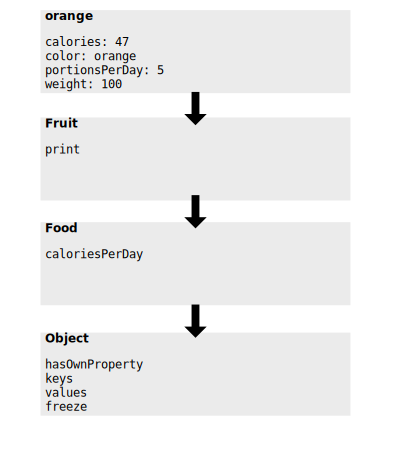
\includegraphics[width=10cm]{prototypechain} 
}
\caption{\label{fig:js-prototypal-chain} Prototypal Chain for Figure \ref{fig:js-prototypal-inheritance}.}
\end{figure} 

\section{Arrays} \label{sec:arrays}
Unlike other languages, JavaScript does not model arrays as continuously indexed tuples. Instead, arrays are a special form of object where the array elements are any value where the property can be coerced to a positive integer number less than 2 \textsuperscript{32} - 1. These array elements are treated differently to regular properties by array prototypes and the length property. 

The length of an array is a property of the array prototype which tracks the highest index in the array. Note, that the highest index of the array does not necessarily track the number of elements in the array; arrays do not enforce any kind of ordering on their properties, making it possible to create a non-contiguous array with `holes' in it. For example \lstinline|let arr = []; arr[0] = 'foo'; arr[2] = 'bar';| produces an array of length 3. The length property is not read-only as one might expect. If one increases length, empty elements will be added to the end of the array, and decreasing the length will truncate the array to satisfy the new length.

Another by-product of arrays being a special form of object is that arrays are not homogeneously typed. Whilst most languages require arrays to only hold values of a single type, JavaScript objects and by extension arrays can contain multiple types of value, as shown by the following example: \lstinline|let array = ['a', 2.0, {}, new Fruit()]|. 

As described above, arrays can have both properties and array elements. If the property fails the array element test described above, then the value is stored as a regular object value. This can lead to subtle bugs when working with numbers if bounds are not checked as values smaller than 0 and greater than 2  \textsuperscript{32} - 1 will not be stored as an array element, as demonstrated in Figure \ref{fig:js-array-max-length}.

\begin{figure}[t]
\begin{lstlisting}
let arr = [];
arr[0] = 'foo'; // array is 
arr.length; // returns 1
arr[4294967296] = 'bar'; // 4294967296 === 2^32-1, property not an element
arr[-1] = 'baz'; // -1 < 0, property not an array element
arr.length; // still returns 1
\end{lstlisting}
\caption{\label{fig:js-array-max-length} Example of Array Object Behaviour.}
\end{figure}

\subsection{Prototype Functions} \label{sec:array-prototype-functions}

\begin{figure}[t]
\begin{lstlisting}
if (!Array.prototype.includes) {
  Object.defineProperty(Array.prototype, 'includes', {
    value: function(needle, index) {
      if (this == null) {
        return false;
      }

      index = index || 0;
      return this.indexOf(needle) > index;
    }
  });
}
\end{lstlisting}
\caption{\label{fig:naive-includes-polyfill} Example of a Naive Includes Polyfill.}
\end{figure}

The array prototype has a large number of helper functions which developers frequently take advantage of, a number of which were added in the latest version of the EMCAScript standard~\cite{EcmaScript}. Table \ref{table:array-prototype} lists some of the more commonly used and interesting functions. As support for the latest ECMAScript standard varies between browsers it can be difficult to developers to judge when it is safe to use a new prototype function however using modern prototype functions typically makes reasoning about code easier. To resolve this tension, developers typically include \textit{polyfills} -- code which copies the behaviour of a prototype function and dynamically adds itself to the prototype if the function is \lstinline|undefined|. Figure \ref{fig:naive-includes-polyfill} contains a naive example implementation of a \lstinline|Array.prototype.includes| polyfill.

\begin{table}[t]
\centering
\begin{tabular}{|p{2cm}|p{4.2cm}|p{9cm}|}
\hline
Function Name & Signature & Description \\ \hline
\lstinline|indexOf| & {\lstinline|indexOf(element)|} & Returns the first index of the array that contains {\lstinline|element|} or -1 if {\lstinline|element|} is not in the array \\ \hline
\lstinline|lastIndexOf| & {\lstinline|lastIndexOf(element)|} & Returns the last index of the array that contains {\lstinline|element|} or -1 if {\lstinline|element|} is not in the array \\ \hline
\lstinline|slice| & {\lstinline|slice(begin, end)|} & Returns a copy of the array with the elements from the index {\lstinline|begin|} up to the {\lstinline|end|} index. If {\lstinline|end|} is not provided it will slice \lstinline|from| {\lstinline|begin|} to the last element of the array \\ \hline
\lstinline|push| & {\lstinline|push(element)|} & Increases the length of the array by one and adds {\lstinline|element|} to the end of the array \\ \hline
\lstinline|pop| & {\lstinline|pop()|} & Removes the last {\lstinline|element|} in the array and returns it \\ \hline
\lstinline|unShift| & {\lstinline|unShift(elementA, elementB, ...)|} & Adds one or more elements to the beginning of an array and returns the new length \\ \hline
\lstinline|includes| & {\lstinline|includes(element, startIndex)|} & Returns \lstinline|true| if the array contains {\lstinline|element|} either starting from {\lstinline|startIndex|} or the start of the array if no {\lstinline|startIndex|} is provided \\ \hline
\lstinline|reverse| & {\lstinline|reverse()|} & Reverses the array in place and returns a reference to the array \\ \hline
\lstinline|forEach| & {\lstinline|forEach(func)|} & Calls {\lstinline|func(value, index, array)|} on each element in the array. \\ \hline
\lstinline|filter| & {\lstinline|filter(func)|} & Returns a new array that contains elements that return \lstinline|true| when {\lstinline|func(currentElement)|} is called on them. \\ \hline
\lstinline|map| & {\lstinline|map(func)|} & Returns a new array with the results of calling {\lstinline|func(value, index, array)|} on each element in the array. \\ \hline
\lstinline|reduce| & {\lstinline|reduce(func,initialValue)|} & Calls {\lstinline|func(accumulator, value, index, array)|} on every element in the array and returns the value of accumulator. If {\lstinline|initialValue|} is provided then the first time {\lstinline|func|} is called then {\lstinline|accumulator|} is set to the value of {\lstinline|initialValue|} \\ \hline
\lstinline|some| & {\lstinline|some(func)|} & Calls {\lstinline|func(element, index, array)|} for every element in the array. Returns \lstinline|true| if {\lstinline|func|} returns \lstinline|true| for at least one element in the array \\ \hline
\lstinline|every| & {\lstinline|every(func)|} & Calls {\lstinline|func(element, index, array)|} for every element in the array. Returns \lstinline|true| if {\lstinline|func|} returns true for all elements in the array \\ \hline
\end{tabular}
\caption{Array Prototype Functions.}
\label{table:array-prototype}
\end{table}

\section{Ensuring Correctness}
Assuring the correctness of JavaScript code is an unsolved problem - in part due to the fact that JavaScript is a dynamically typed scripting language but also due to legacy design decisions. Efforts have been made to make the language itself safer to use, for example ECMAScript 5 introduced a strict mode (later made the default mode in ECMAScript 6) which restricts the use of certain language features and also defines additional circumstances in which exceptions should be thrown. However there are still many subtle errors that can occur even within the safer subset of JavaScript.

Tools like Eslint and Flow are commonly used by developers to statically analyse code and identify bugs but are limited in their scope. Eslint uses a narrow set of rules to identify possibly dangerous behaviour. Flow is constrained to reasoning about types and in some cases requires additional code annotation to identify possible errors. These limited sets of warnings do not fully reflect the dynamic nature of JavaScript and the subtle interactions that can occur due to prototypal inheritance, dynamic property access, and dynamic dispatch. There have been a number of attempts to analyse JavaScript statically however most approaches fall short of useful due to their inability to reason about functions like \lstinline{call()} and \lstinline{apply()}~\cite{sridharan2012correlation}, with the best results requiring an element of dynamic analysis as well~\cite{logozzo2010rata, wei2013practical}.

Consequently there has been a shift in interest towards analysing safer (and less dynamic) targets which compile to JavaScript, the most popular of which is Typescript. Typescript is a superset of ECMAScript 6 which includes optional types to enable errors to be caught statically before compilation. Although TypeScript makes it easier to reason about potential errors caused by coercion, TypeScript itself provides no guarantees of static soundness - it is still possible for a TypeScript program to compile to JavaScript successfully and encounter a run-time error as a result of type coercion when executed~\cite{bierman2014understanding}. Extensions to TypeScript have been suggested to provide soundness ~\cite{richards2015concrete, DBLP:conf/popl/2015} although these approaches require a modified interpreter or runtime enforcement. Regardless, whilst TypeScript and its derivatives provide a way of reducing or eliminating type based errors they do not help identify or eliminate errors that occur due to other dynamic features of JavaScript such as prototypal inheritance, dynamic property access, or dynamic dispatch.

There have been a number of attempts to produce formal semantics for JavaScript, to allow for better reasoning about JavaScript code, however no attempts can be considered completely successful. One approach taken is to translate a subset of the JavaScript language (targeting ECMAScript 5 in strict mode) to an intermediate language, JSL, on which analysis can be performed ~\cite{gardner2012towards}. Although the results of this type of analysis is promising, the process and toolchain requires an expert level understanding of the semantics of JavaScript and also requires developers to annotate their code pre and post-conditions. While, this approach may be suited for smaller programs (or critical subsets of programs) its approach does not scale well to large applications. Other approaches such a KJS~\cite{park2015kjs} and \ensuremath{\lambda}JS\cite{guha2010essence} support even less of the language than JaVerT and crucially none of the three approaches target, or can be easily extended to, the ECMAScript 6 specification.

Symbolic execution is a good match for JavaScript. By concretely executing the program, reasoning about the dynamic nature of JavaScript is deferred to the interpreter. The use of an interpreter for testing also provides flexibility. If JavaScript needs to be tested in another environment, switching interpreter is a relatively easy change to make. Additionally, concrete execution comes without the penalty of having to model the entire language specification as any non-modelled function can simply revert to concrete execution.

\chapter{Implementation} \label{sec:implementation}

ExpoSE~\cite{DBLP:conf/spin/2017} is a recently developed tool for dynamic symbolic execution of JavaScript. It takes a program as input and attempts explore all feasible paths in the program up to a maximum path count or until it exceeds a maximum time limit. Programs are instrumented using Jalangi2, a framework that provides callbacks for JavaScript statements which are used to build the symbolic representation of the program. New inputs are generated by solving path constraints using the Z3 SMT solver~\cite{de2008z3}.

Below I outline the implementation of my extensions to ExpoSE to support arrays. Specifically I describe the challenges in encoding JavaScript arrays in Z3, the modifications necessary to symbolically reason about arrays and their length, and a description of the function models I have written for Array prototype functions.

\section{JavaScript Array Encoding}
Z3 supports two array-like theories: the theory of arrays and the theory of sequences which provided a choice for which theory to encode JavaScript arrays in. Z3 offers a rich number of operations on sequences including obtaining the length, concatenating sequences, and checking whether an element is in a sequence. Conversely, the theory of array support is limited to three basic operations: select, store, and map. Initially sequences seemed like a more natural fit as many array prototype functions map naturally to Z3 sequence operations. For instance, \lstinline|Z3_mk_seq_contains| is very similar to \lstinline|Array.prototype.includes| and \lstinline|Z3_mk_seq_index| is similar to to \lstinline|Array.prototype.indexOf|. However after experimentation it became clear that concretising sequences was impossible as extracting single elements from a sequence produced a unit sequence rather than the value of the element. As a result of being unable to concretise sequences, JavaScript arrays are encoded using Z3’s array theory. 

Z3 arrays are one dimensional unbounded maps where the index and values both have a \textit{sort}, Z3's terminology for type. Read and write operations on the array are mapped to select and store axioms respectively where the relationship between select and store is defined by $select(store(a, i, v), i) = v$ where $a$ is an array, $i$ is an array index, and $v$ is a value. Due to their unbounded and strongly typed nature, Z3 arrays do not directly correspond to JavaScript arrays which, as described in Section~\ref{sec:arrays}, can contain multiple types, are bounded between the indices 0 and 2\textsuperscript{32}-1, and have a mutable length. As a result certain tradeoffs have to be made in the way arrays are modelled and encoded. The first limitation is that arrays are only able to be symbolically modelled if they are initialised with values of a single type and only if the type of the values have an analogous Z3 sort which limits the types that are supported to booleans, numbers, and strings. The second limitation is that holes that are created by mutating the length of an array or setting values non-sequentially are not modelled. Finally, in order to encode the finite length of JavaScript arrays, for each Z3 array a separate Z3 integer variable is required represents the length of the array. 

\subsection{Representing Array Length}
When the array is created an assertion $Length > 0$ is made. Whenever the concrete JavaScript array is accessed, if the index, $i$, is within the bounds of the concrete array then an assertion $i > 0 \land i < Length$ is made, implying that the array's length is greater than the symbolic index. If the index is not within the bounds of the concrete array then the assertion $\lnot{(i \geq 0 \land i < Length)}$ is made, which implies that the symbolic length is less than the accessed index. When the array is pushed to and popped from, a new length variable is created and the length is asserted to be the previous length plus or minus one. When the array is set to, a fresh length variable is created and an assertion $Length < i$ is made. When the array length is directly set to, \lstinline|{array.length = x;| a fresh length variable is created and an assertion $Length = x$ is made, where $x$ is the value that was set.

Consider the example program in Figure \ref{fig:expose-array-length} which demonstrates the constraints on the symbolic length of an array as it is accessed and updated. Initially, (line 2) the length of the array is constrained only to be greater or equal to 0, effectively unbounded. On line 3, the array is accessed at index 0 and the constraint then changes to have a length greater than the accessed value as the concrete array (\lstinline|['a']|) has an item at that index. On line 4, the array is pushed to and a new Z3 variable is created to model the length of the array but the constraint still depends on the previous variable - the new constraint is the previous variable's constraints plus one. On line 5 the array is accessed out of bounds and a new assertion is made that the length is less than the out of bounds index. When the array is set on line 6 another fresh Z3 variable is used to model the length of the array but this does not depend on the previous variable, instead it asserts that the length is greater than the accessed index (20). On line 7 the array is popped from, and similarly to line 4 when the array was pushed, a new length variable is created than depends on the previous variable's constraints minus one.

\begin{figure}[t]
\lstinputlisting{array_manipulation.js}
\caption{\label{fig:expose-array-length} Example of Array Constraints Enforcement.}
\end{figure}

\section{Array Support Architecture}
ExpoSE is architected as a number of distinct modules: Z3JS, a JavaScript interface to Z3’s C API, the Distributor, a highly parallelised dispatcher for symbolic execution paths and an aggregator of information, the Analyser, which executes the symbolic analysis for a given path, and the Tester, which automatically runs ExpoSE’s unit tests. The bulk of my work, was done in the Analyser and Z3JS. Below I briefly outline the modifications that were made to each.

\subsection{Z3JS}
Z3JS provides an interface between the Z3’s C API and JavaScript. Its main components are a \lstinline|Solver| class, a \lstinline|Query| class, a \lstinline|Model| class, an \lstinline|Expr| class, and a \lstinline|Context|~class. The \lstinline|Context| class wraps the Z3 context and acts as a facade for the Z3 API calls. The \lstinline|Expr| class wraps constructed Z3 expressions and has helper functions for printing and creating a concrete value from the symbolic expression. The \lstinline|Model| class wraps Z3 model objects and the query class is used to request solutions for models from Z3.

In order to be able to interface with Z3’s array functions I had to add a number of functions to the context class including \lstinline|mkArray|, \lstinline|mkSelect|, \lstinline|mkStore| as well as functions used to perform assertions using quantifiers, \lstinline|mkForAll| and \lstinline|mkExists|. The quantifier based functions expect arrays to be passed as parameters so I also had to change some helper functions \lstinline|_buildChecks()| and \lstinline|Z3Utils.astArray()| to work with arrays of parameters.

I modified \lstinline|Expr| to a hold of number of array specific properties that need to be required throughout ExpoSE such as the expression for array length, the type of the array, the start index of the array (described in detail in Section \ref{slice-function-model}), the name of the array, and a counter for the number of length expressions an array has. All of these properties have getter functions and either an increment function or a setter. I have also written helper functions to hide the complexity of storing to \lstinline|setAtIndex()| and selecting from (\lstinline|selectFromIndex()|) an array expression.

A key function in \lstinline|Expr| is \lstinline|asConstant()| which turns the expression into a concrete value. I rewrote the function into a small switch statement which evaluates the sort of the expression. To be able to support turning array expressions into constants I had to be able to get a constant value for the expression which represents the length of the array. In order to do that I had to change the signature of the function to accept a model, using which I can call \lstinline|model.eval()| to get an interpretation for the expression. Using the concrete value for the length I can then iterate for the length of the array calling \lstinline|selectFromIndex()| to produce a concrete JavaScript array of values.

\subsection{Analyser}
SymbolicState.js has a number of functions that are called when a symbolic value is used during execution. \lstinline|createSymbolicValue()| has been modified to check if the concrete type is either homogeneously typed or an empty array, if so Z3JS’s \lstinline|context.mkArray()| is called to create the array, with the correct homogeneous type, and assertions are made about the array’s length, as described above, to keep the array bounded.

\lstinline|symbolicField()| has been modified to check if the array is being accessed with a potentially valid array index - i.e. a number between 0 and 2\textsuperscript{32}-1. If so, assertions are made about the length, as described above, and if the index is less than the array length Z3JS’s \lstinline|Expr.selectFromIndex()| is called. The assertions about the array length are pushed using \lstinline|symbolicConditional()| which pushes either an expression, or the negation of that expression, depending on the result of a concrete condition - consequently whenever an in-bounds array access occurs, \lstinline|let arr = [0, 1, 2]; arr[1];|, a new path will be created to explore an out of bounds access and vice versa. \lstinline|symbolicField()| has also been modified to return the expression for the array's length when the \lstinline|length| property is accessed.

\lstinline|putField()| has been modified, in SymbolicExecution.js, to call \lstinline|symbolicSetField()|, a new function in SymbolicState.js, if the concrete value \lstinline|putField()| is called on is an array. \lstinline|symbolicSetField()| has two cases: if the field is a valid array index then the value is stored in the array and a new length variable is create, alternatively if the \lstinline|.length| field is assigned to then the value is set as the new length.

\subsection{Function Models}
\begin{figure}[t]
\lstinputlisting{naive_includes_model.js}
\caption{\label{fig:naive-includes} Example of a Naive Implementation of a Function Model for Includes.}
\end{figure}

When symbolic values are used in native %prototype functions (such as those in \lstinline{Array.prototype} described in Section \ref{sec:array-prototype-functions}) they leave the environment in which the program is being analysed and consequently become concretised preventing new paths from being explored from that point onwards in the program. This results in incomplete exploration and a reduction in code coverage. One solution to this problem is to clone the behaviour of functions in native JavaScript, Figure~\ref{fig:naive-includes} shows an example of how this might be achieved. Although this approach achieves the goal of obtaining a symbolic representation of the result of the function it also creates additional paths for each branching condition or loop inside the function. An alternative solution to this problem is to model the behaviour of the function. Doing this is typically more time consuming but has the advantage of avoiding path explosion and deferring the cost to the SMT solver.

ExpoSE has a framework for modelling prototype functions in the \lstinline|FunctionModel| module. Prototypes in the \lstinline|FunctionModel| module are exposed as a symbolic hook that concretely executes the prototype function and then if a condition is met also symbolically executes a model function if it exists. 
%TODO make it clear that these are not the only function models
Below I provide a detailed look at some of the function models that have been implemented including for \lstinline|slice|, \lstinline|indexOf|, and \lstinline|push|.

\textbf{slice} \label{slice-function-model}
\begin{figure}[t]
\begin{lstlisting}
models[Array.prototype.slice] = symbolicHook(
            (c, _f, base, args, _r) => c.state.isSymbolic(base) && c.state.getConcrete(base) instanceof Array,
            (c, _f, base, args, result) => {
                const ctx = c.state.ctx;
                const array = c.state.asSymbolic(base);
                let begin = args[0] ? c.state.asSymbolic(args[0]) : ctx.mkIntVal(0);
                let end = args[1] ? c.state.asSymbolic(args[1]) : array.getLength();

                // handle slice(-1)
                // if begin is less than 0, begin equals 0 and end equals arg[0], else begin must be ge than 0
                c.state.pushCondition(ctx.mkIte(
                    ctx.mkLt(begin, ctx.mkIntVal(0)), 
                    ctx.mkAnd(ctx.mkEq(begin, ctx.mkIntVal(0)), ctx.mkEq(end, c.state.asSymbolic(args[0]))),
                    ctx.mkGe(begin, ctx.mkIntVal(0))
                ));

                // end cannot be greater than array length
                c.state.pushCondition(ctx.mkLe(end, array.getLength()), true);

                // This clones the array in Z3 by doing a store that stores the same value at the index
                const noOpIndex = ctx.mkIntVal(0);
                const copiedArray = array.setAtIndex(noOpIndex, array.selectFromIndex(noOpIndex));
                
                const newLength = ctx.mkIntVar(`${array.getName()}_Length_${array.incrementLengthCounter()}`);
                copiedArray.setLength(newLength);
                copiedArray.increaseStartIndex(begin);

                /* The new length should be greater than 0 AND 
                   IF end is positive, less than or equal to end's length -> slice(0, 4)
                   ELSE, less than or equal to the old length-end -> slice(0, -1) */
                c.state.pushCondition(
                    ctx.mkAnd(
                        ctx.mkGe(newLength, ctx.mkIntVal(0)), 
                        ctx.mkIte(
                            ctx.mkGe(end, ctx.mkIntVal(0)), 
                            ctx.mkLe(newLength, ctx.mkSub(array.getLength(), end)),
                            // negative end indexing 
                            ctx.mkLe(newLength, ctx.mkSub(array.getLength(), ctx.mkAdd(end, begin)))
                        )
                    ),
                    true
                );
                return new ConcolicValue(result, copiedArray);             
            }
        );
\end{lstlisting}
\caption{\label{fig:slice-func-model} Slice Function Model.}
\end{figure}

\lstinline|Array.prototype.slice| returns a shallow copy of a subsection of array. It takes two optional parameters \lstinline|begin| which marks the start index for the shallow copy to begin from and \lstinline|end| which marks the first index in the array that should not be included in the shallow copy. Both parameters also accept negative indices which are interpreted as reverse indexing. If no \lstinline{begin} parameter is passed then \lstinline{slice} returns a full copy of the array.

The function model for \lstinline|slice| is shown in Figure~\ref{fig:slice-func-model}. The first function passed to the \lstinline|symbolicHook| checks that the function the prototype is called on is a symbolic array as the \lstinline|slice| function can also be used on strings. The second function passed to the \lstinline|symbolicHook| models the function. Lines 4-18 check which arguments are passed to the function, set the default parameters if necessary, and perform validation. Validation is performed by asserting that if the first argument is negative that \lstinline|begin| should be 0 and \lstinline|end| should be set to the value of the first argument, as this is a negative indexing operation. Lines 21-22 create a shallow copy of the array by performing a store with no effect and lines 24-26 create a new variable to represent the new array's length. Line 26 increases the \textit{start index} of the copied array - the start index is the pointer to the first index of the unbounded Z3 which should be considered part of the array that is being symbolically modelled. This methodology allows for an arbitrary number of slices to be made by continually incrementing the pointer. Both \lstinline|Expr.selectFromIndex()| and \lstinline|Expr.setAtIndex()| use the start index offset hiding the complexity of accounting for the start index pointer in most cases but in the \lstinline|FunctionModels| module, where the helper functions, the start index needs to be taken into account. Lines 31-42 describe assertions on the length of the new array. The length must be greater or equal to 0 and if \lstinline|end| is positive, the length of the copied array is $end - start$, else the new array length is $oldArrayLength - (end + begin)$.

This model allows for all but one of the acceptable signatures of \lstinline|slice| including \lstinline|slice()|, \lstinline|slice(-1)|, and \lstinline|slice(1, -2)| but excluding \lstinline|slice(4, 1)| -- which would return an empty array.

\textbf{pop}
\begin{figure}[t]
\begin{lstlisting}
models[Array.prototype.pop] = symbolicHook(
            (c, _f, base, args, _r) => c.state.isSymbolic(base) && c.state.getConcrete(base) instanceof Array,
            (c, _f, base, args, result) => {
                const ctx = c.state.ctx;
                const array = c.state.asSymbolic(base);

                const oldLength = array.getLength();
                const newLength = ctx.mkIntVar(`${array.getName()}_Length_${array.incrementLengthCounter()}`);

                const value = new ConcolicValue(result, array.selectFromIndex(oldLength));
                c.state.pushCondition(ctx.mkEq(newLength, ctx.mkSub(oldLength, ctx.mkIntVal(1))), true);
                
                array.setLength(newLength);
                return value;
            }
        );
\end{lstlisting}
\caption{\label{fig:pop-func-model} Pop Function Model.}
\end{figure}

\lstinline|Array.prototype.pop| returns the element at the last index of the array and reduces its length by one. The function model for \lstinline|pop| is shown in Figure~\ref{fig:pop-func-model}. Line 2, included in every function model, checks that the \lstinline|base| argument is symbolic and an array - if so the second function starting on line 3 is called. Lines 4-8 create a new Z3 variable to store the new length, and create a temporary variable to store the old length. Line 10 fetches the value to be popped from the array and lines 11-13 set the new length to one less than the previous length and assign it to the array expression. The popped value is then returned.

%TODO describe indexOf

\subsection{Tests}
\begin{figure}[t]
\begin{lstlisting}
var q = symbolic UnderTest initial [0, 1, 1, 4, 4, 1];

// Clone the length
var length = q.length;
if (q.length === 3) {
  q.length = 42;
  if (q.length === 42) {
    console.log('Success');
  } else {
    throw 'array_set_length: This should be unreachable';
  }
}
\end{lstlisting}
\caption{\label{fig:example-length-test} Example Unit Test.}
\end{figure}

All of the array functionality implemented, including function models and the regular concrete behaviour of arrays, is backed by a number of tests. Tests are written in a way to prompt to ExpoSE to attempt to generate inputs which would explore infeasible paths, as demonstrated in Figure~\ref{fig:example-length-test}. The expected number of errors are recorded in an array specific test runner and if the number of errors thrown does not match then the test runner rethrows the error indicating a change in behaviour. The array-specific test suite is run as a git pre-push hook to act as a smoke test and prevent regressions being committed to the repository.

\chapter{Evaluation}
To evaluate the extensions to ExpoSE I have tested two popular JavaScript libraries, \lstinline|Lodash/array| and \lstinline|Minimist|. Both libraries have roughly 14 million downloads a week from npm and make extensive use of array operations making them ideal targets to evaluate. I also present a methodology for verification of array polyfills using ExpoSE using which I discover bugs in a popular polyfill library.

\section{Methodology}
Using a version of ExpoSE with support for numbers, strings, Booleans, \lstinline|undefined|, \lstinline|null| and the extensions for array support described in Section \ref{sec:implementation} I symbolically executed \lstinline|Minimist| and \lstinline|Lodash/array| with and without array support enabled. \lstinline|Minimist| was tested with a simple harness as the module is exported as a single function and \lstinline|Lodash/array| was tested with ExpoSE's harness generator which explores all the public functions in a library with symbolic arguments of all supported types. Tests were run on the same machine with 264GB of RAM and an Intel Xeon 6142 @ 2.6GHz CPU with 64 cores. Tests were left to run until they exhausted all paths, hit a max path count of 1,000,000 or ran for 15 minutes. Impact is measured in the amount of coverage gained with array support enabled, the number of additional paths generated, as well as the increase in time taken.

\section{Results}
\begin{table}[t]
\centering
\begin{tabular}{|p{4cm}|p{2cm}|p{2cm}|p{2cm}|p{2cm}|}
\hline
& \lstinline|Minimist| with Arrays Disabled & \lstinline|Minimist| & \lstinline|Lodash/array| with Arrays Disabled & \lstinline|Lodash/array| \\ \hline
Lines Covered & 34\% & 73\% & 82.6\% & 83\% \\ \hline
%Terms Covered & 22\% & 64\% & 75.8\% & 76.4\% \\ \hline
Total Test Duration & 902s & 901s & 376s & 801s \\ \hline
Median Test Case Duration & 6.49s & 5.42s & 7.17s & 9.63s \\ \hline
90\textsuperscript{th} Percentile Test Case Duration & 9.7s & 21.93s & 10.75s & 11.55s \\ \hline
Max Test Case Duration & 215.93s & 315.33s & 14.8s & 17.41s \\ \hline
Total Paths Explored & 7243 & 2015 & 2450 & 5101 \\ \hline
\end{tabular}
\caption{Results.}
\label{table:results}
\end{table}

%TODO Get graphs and discuss more
The results in Table \ref{table:results} show a clear difference in behaviour of the two libraries that are tested, although both have a net gain in coverage. \lstinline|Minimist| has a drastic jump in coverage with array support enabled which comes at the cost of total path count. The number of paths appears to be reduced as the execution was constrained by time, rather than a reduction in a number of feasible paths. The combination of a low path count and the high max and 90\textsuperscript{th} percentile test case duration indicates a small number of large queries which suggests that ExpoSE had large path constraints, potentially as a result of deeper exploration of the program. \lstinline|Lodash/array| exhibited different behaviour, whilst it only received a small bump in coverage it more than doubled the number of paths explored and spent on average ~30\% longer on each path. 


% Section Concretisation
Examining why the jump in coverage was so small revealed that the majority of functions accept strings. The remaining uncovered areas of \lstinline|Lodash/array| mostly relate to internal functions which are unreachable from the \lstinline|Lodash/array| module and polyfill code. Both libraries have areas that concretise due to lack of Object support.


% Array performance

% Limitations of methodology
Overall the increased cost in query time appears to be a reasonable trade-off for the net gain in terms of both coverage and additional paths to explore although there is reason to be concerned about the performance of arrays on particular deep paths with many assertions as demonstrated by the large increase (100s) in max test case duration of \lstinline|Minimist|.

\section{Polyfill Verification}
Array polyfills, as discussed in \ref{sec:array-prototype-functions}, attempt to mimic the behaviour of standard prototype functions for backwards compatibility purposes. By giving symbolic input to both a polyfill and the standard implementation function and comparing the result deviations in behaviour can be identified. Below I present an example harness and describe a bug found in a popular polyfill library.

\begin{figure}[t]
\lstinputlisting{polyfill_harness.js}
\caption{\label{fig:polyfill-test-harness} Polyfill Test Harness.}
\end{figure}

The harness, shown in \ref{fig:polyfill-test-harness}, calls the function \lstinline|testPolyfill()| with the polyfill function under test, the matching standard function, a symbolic \lstinline|thisArg| argument, and an array of symbolic values. The \lstinline|thisArg| argument is the argument that represents the value that the prototype is being invoked from, the \lstinline|arr| in \lstinline|arr.includes(myValue, 0);|. The array of symbolic values are the values that should be passed to the function. \lstinline|testPolyfill()| then uses \lstinline|apply()| to call the two functions, using \lstinline|try| to prevent an exception from causing the test case to fail, and stores the results. If the results differ then an exception is thrown which contains a string representation of the two values and the key word alert to make the output easily to identify using \lstinline|grep|.

\lstinline|js-polyfills| is a popular polyfill library with 970 stars on Github and 7,000 weekly downloads. It contains polyfills for many array functions including \lstinline|Array.includes|. Using the harness and techniques described above, ExpoSE identified that calling the \lstinline|includes| polyfill with an \lstinline|undefined| base type would cause the function to return \lstinline|false| whereas the standard prototype implementation throws an exception. If a program used a pattern like \lstinline|try {array.includes(a)} catch (e) {...}| to do error handling in the case of being passed an undefined array then as a result of this bug the program would function differently in a polyfilled environment.

\chapter{Conclusion}
In this report I have presented an encoding of JavaScript arrays using the Z3 SMT solver. I also discussed the implementation of extensions to ExpoSE to support arrays including example models for popular array prototype functions. I also demonstrated that the extensions to ExpoSE are effective at increasing coverage on programs that use arrays with a reasonable increase in time spent solving and demonstrate a case where as a result of the implementation ExpoSE is able to find a bug in a popular polyfill library.

%section extensions
There are many possible extensions to the work presented in this report. The most natural extension would be to explore supporting non-homogeneous arrays, which could be achieved through encoding an array as seven Z3 boolean arrays, one for each JavaScript type plus an additional array to encode which array an element exists in. This approach leans heavily on Z3 and would likely come with a large performance cost. Another extension would be to extend homogeneous arrays to support holes, a naive approach would be to store a `magic value' at indices that should contain a hole however this approach would only work for String and Number arrays. A more advanced approach could add an uninterpreted function to array expressions which would indicate the indices in the array that should contain holes. Another limitation of the current implementation is that pure symbols only attempt to use arrays of strings -- a more advanced implementation could attempt to use an array of each supported type and an empty array.

%section challenges encountered

%section reflection on areas of improvement
I believe that if I was to tackle another project working with a symbolic execution engine I would approach it differently. Rather than relying exclusively on micro-programs for regression testing I would also write a number of real-world-esque programs in the region of 50-200 lines of code. I found that there were some bugs in my implementation that were not picked up early by my test cases and but became apparent testing \lstinline|Minimist|. I would also approach implementation differently - early on I was afraid to touch too many parts of the program for fear of breaking existing features however I came to realise that the combination of the way  ExpoSE is designed and arrays being a somewhat special case means that often the cleanest implementation of solutions sometimes require a change that spans across multiple modules. I would also write code more defensively and with more verbose logging. I encountered two major bugs which I invested several days into which could have been prevented if I had. The first bug was that \lstinline|Array.prototype.slice| is also used reused for strings however I was not checking in my prototype functions that the \lstinline|this| argument was actually an array, had I written my code more defensively then this would not have been an issue. Another bug I identified was that my put field method was silently failing to be called as it was being called with concrete arguments -- a more liberal use of logging would have made this much easier to track down. JavaScript is a language that has a lot of edge cases and  writing code assuming it may fail seems to be a good motto.

The biggest challenge for me in the project, and a source of great frustration, was modelling functions in Z3's SMT-LIB syntax. I frequently made errors in my assumptions, misunderstood the way in which assertions interacted, and struggled with mixing quantifiers. Once I moved to modelling entirely in Z3JS I found the process much easier but I believe this may have been at the expense of a richer understanding of how SMT works.

Overall I believe the project was a success and I am proud of the contributions I have presented.

\newpage
\bibliography{/Users/arran/Documents/Github/FullUnit_1718_ArranFrance/Report/bibliography}
\bibliographystyle{ieeetr}
\label{endpage}

\newpage

\chapter{Appendix}

\section{Professional Issues}
It is possible to imagine a world in which ExpoSE is deployed as a tool to automatically test open source code from GitHub or npm, either as part of a survey of open source JavaScript software or as a free service. Similar tools already exist such as Snyk, which attempts to find dependencies with known vulnerabilities, and the static analysis tool Deepscan, which attempts to find common coding errors. In such a situation it would be important to consider how the process of disclosing a a bug would work, given that ExpoSE has no framework for identifying the severity or impact of the bugs it finds, and the difficulty in doing so reliably~\cite{lamkanfi2010predicting}. Whilst ExpoSE cannot produce false positives, the impact of a bug found by it can range from a low impact bug that is unlikely to be triggered to a serious security vulnerability. 

The steps to take to disclose a flaw ethically are not universally agreed upon and existing literature mainly deals with security vulnerabilities due to their critical nature. There are two broad types of disclosure that could qualify as ethical. The first is \textit{full disclosure}, in which the bug is reported as early and widely as possible with the intent of informing end users about the flaw. The second is \textit{responsible disclosure}, in which the flaw is reported to the maintainer or vendor and no one else until the flaw is rectified. Whilst the definition of full disclosure is concrete, the definition of responsible disclosure is more ambiguous and provokes a number of questions. What do you do if the flaw is not rectified? At what point does the risk of potential harm require you to release the details of the vulnerability to the public? Does the amount of time given vary with the severity of the bug? These questions, and the discussion about the best method for disclosure, are still active areas of debate today. This debate, and the issues with the boilerplate definition of responsible disclosure, is highlighted by two high profile vulnerabilities disclosed this year. 

The Meltdown and Spectre vulnerabilities, which revealed underlying flaws in the methods for speculative execution in CPUs across multiple vendors, were announced in January. Given the nature of the vulnerability numerous parties were required to know about the flaw, including operating system and browser vendors as well as cloud computing platforms such as AWS and Azure. The additional complexity created by the number of groups involved resulted in a chaotic public disclosure due to a broken embargo. The number of parties involved also had a drastic effect on the timeline of discovery to disclosure. Google's Project Zero, the team behind the initial discovery, have a standard 90 day window after which they disclose but, due to the complexity of the vulnerability and the number of groups involved, this was doubled to 6 months.

Whilst the Meltdown and Spectre vulnerabilities are clearly extraordinary circumstances they highlight one of the issues with the standard model of responsible disclosure - a long period where users are unknowingly affected and vulnerable to exploitation.

Another high profile vulnerability disclosed this year was the High Sierra Mac OS login bypass which enabled users to access root privileges without a password. The bug was discovered by Lemi Ergin and was disclosed via Twitter leading him to face criticism for failing to follow responsible disclosure principles. Whilst it is not considered good practise to not work with the vendor when disclosing a vulnerability, Ergin's tweet prompted Apple to release a next day update whilst Ergin's company's email earlier in the week and a post on Apple's Developer Forum failed to prompt action~\cite{ergin-disclosure}.

Whilst most professionals would broadly agree that responsible disclosure is the preferred method, there are respected individuals within the security field such as Bruce Schneier that argue in favour of full disclosure~\cite{debating-full-disclosure}. He argues that ``public scrutiny is how security improves" and that it is important that consumers have ``all the information" to ``make an informed decision about security".

I think it is worth re-evaluating the loaded term of responsible disclosure and examining what, if any, role full disclosure has to play. It is clear from the Ergin's tweet that full disclosure produces results, but at what risk? A common argument made in favour of responsible disclosure is that sharing the details of a vulnerability is irresponsible - that the `bad guys' can abuse them if they're made public. Schneier argues that malicious users are often more advanced than security researchers and may already know about the vulnerability and be actively exploiting it. In addition, if malciious actors are not aware of the vulnerability - Schneider suggests that releasing the details of a vulnerability is a reasonable trade-off for the increased visibility of the risk that users have. Conversely security professional Troy Hunt, creator of the data breach service \lstinline{of have i been pwned?}, argues that public disclosure is not appropriate if it would immediately increase the risk to users~\cite{responsibility-of-public-disclosure}. However, in cases where responsible disclosure is made difficult by unwilling disclosure recipients (and in cases with organisations and individuals who have a poor track record of responding to disclosures), Hunt believes it is in the public's interest to perform full disclosure~\cite{kids-pass-responsible-disclosure}.

Google's Project Zero, the security research team that initially identified the Spectre and Meltdown vulnerabilities, have also struggled to identify the best way to handle disclosure. They received criticism for their strict handling of a vulnerability that they discovered in Windows 7 which was publicly disclosed two days before a patch was released by Microsoft. As a result of the backlash Project Zero added a 14 day grace period to their 90 day disclosure policy but they also make provision for certain ``extreme circumstances””, in which they reserve the right to bring the deadline forward or backwards~\cite{project-zero-update-policy}. In doing so they acknowledge the complexity of disclosing security vulnerabilities.

In conclusion, when considering how to responsibly disclose I believe there are a number of factors that must be considered: the risk to users, the number of organisations that need to be involved, the vendor's history of compliance, and if there are known exploits for the vulnerability already being used. I reject the notion that there is a `one size fits all' approach to responsible disclosure and suggest that, whilst full disclosure should not be the default course of action, it warrants consideration in situations when disclosure would present no risk to users or when dealing with organisations or individuals who have a history of non-compliance.

My conclusion prompts the question: how can responsible disclosure be achieved in the hypothetical world in which ExpoSE is deployed as an automated tool to discover bugs? I believe that every bug found would have to be treated as a possible vulnerability and be reported privately to the maintainer. I would provide a 90 day window for response, after which I would post the vulnerability to a public issue tracker and attempt to alert any public codebases which depended on that code.

\end{document}

\end{article}
